\chapter{Basic Quantum Algorithms}

This chapter presents three foundational quantum algorithms: \begin{itemize}
	\item Deutsch's algorithm, 
	\item the Deutsch--Jozsa algorithm, and 
	\item the Bernstein--Vazirani algorithm.
\end{itemize} Each illustrates how quantum interference and phase‐kickback enable exponential or polynomial speedups over classical counterparts.

\section{Deutsch's Algorithm}\label{sec:Deutsch}
\subsection{Problem Statement}
\begin{definition}[Boolean Oracle Problem]
	Let $f:\{0,1\}\to\{0,1\}$ be a black‐box Boolean function.  We are promised that $f$ is either \emph{constant} (i.e.\ $f(0)=f(1)$) or \emph{balanced} (i.e.\ $f(0)\neq f(1)$).  The goal is to decide which case holds using as few queries to $f$ as possible.
\end{definition}
\begin{figure}[ht]
	\centering
	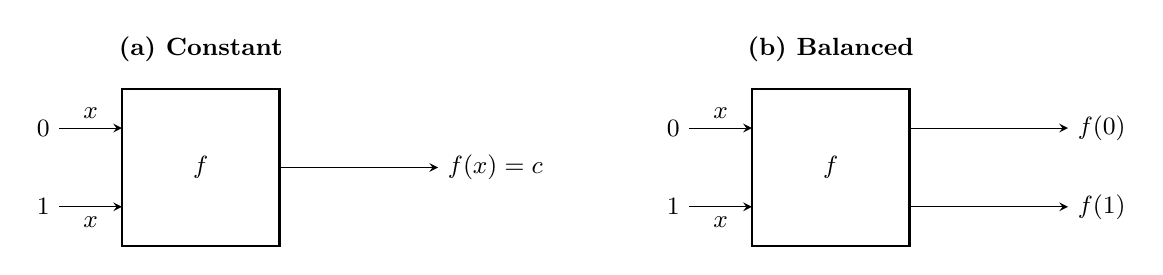
\begin{tikzpicture}[>=stealth, every node/.style={font=\small}]
		% Constant case
		\begin{scope}
			\node at (0,1.5) {\bfseries (a) Constant};
			% inputs
			\node (in0) at (-2,0.5) {$0$};
			\node (in1) at (-2,-0.5) {$1$};
			\draw[->] (in0) -- (-1,0.5) node[midway,above] {$x$};
			\draw[->] (in1) -- (-1,-0.5) node[midway,below] {$x$};
			% oracle box
			\node[draw, thick, minimum width=2cm, minimum height=2cm] (oracle) at (0,0) {$f$};
			% outputs (same)
			\draw[->] (oracle.east|-0.5,0) -- +(2,0) node[right] {$f(x)=c$};
		\end{scope}
		
		% Balanced case
		\begin{scope}[xshift=8cm]
			\node at (0,1.5) {\bfseries (b) Balanced};
			% inputs
			\node (in0b) at (-2,0.5) {$0$};
			\node (in1b) at (-2,-0.5) {$1$};
			\draw[->] (in0b) -- (-1,0.5) node[midway,above] {$x$};
			\draw[->] (in1b) -- (-1,-0.5) node[midway,below] {$x$};
			% oracle box
			\node[draw, thick, minimum width=2cm, minimum height=2cm] (oracleb) at (0,0) {$f$};
			% outputs (different)
			\draw[->] (oracleb.east|-0.5,0.5) -- +(2,0) node[right] {$f(0)$};
			\draw[->] (oracleb.east|-0.5,-0.5) -- +(2,0) node[right] {$f(1)$};
		\end{scope}
%		% Caption label
%		\node[below=3cm of $(0,0)$, align=center] {
%			\small A black‐box Boolean function $\{0,1\}\to\{0,1\}$, with (a) constant ($f(0)=f(1)=c$) and (b) balanced ($f(0)\neq f(1)$) cases.
%		};
	\end{tikzpicture}
	\caption{Oracle for the constant vs.\ balanced promise problem.}
\end{figure}
Classically, one must query both $f(0)$ and $f(1)$ to distinguish the two cases, yielding a lower bound of two queries.  Deutsch’s quantum algorithm achieves a one‐query solution by exploiting superposition and interference.

\newpage
\subsection{Quantum Oracle Model}
\begin{definition}[Oracle Unitary on Two Qubits]
	Given a Boolean function $f:\{0,1\}\to\{0,1\}$, the associated \emph{oracle unitary} is the linear operator \[
	\fullfunction{U_f}{\mathbb C^4}{\mathbb C^4}{\ket{x,y}}{\ket{x,y\oplus f(x)}},
	\] where $\C^4=\C^2\otimes\C^2$ is the two-qubit Hilbert space and $x,y\in\{0,1\}$. This preserves unitarity and acts trivially on superpositions.
\end{definition}
\vfill
\begin{example}
Given $U_f:\C^4\to \C^4:\ket{x,y}\mapsto\ket{x,y\oplus f(x)}$, consider : \begin{center}
	\begin{quantikz}[column sep=.5cm]
		\lstick{$\ket{0}$} & \qw      & \qw                              &\gate[2]{U_f} & \qw & \push{\scriptstyle \ket{0}\oplus f(H\ket{0})} \qw & \qw \\
		\lstick{$\ket{0}$} & \gate{H} & \push{\scriptstyle H\ket{0}} \qw &              & \qw & \push{\scriptstyle H\ket{0}} \qw & \qw
	\end{quantikz}
\end{center} Then \begin{align*}
U_f(H\ket{0},\ket{0}) = U_f\bigl(\ket{+}\otimes\ket0\bigr)=
U_f\left(\tfrac{\ket0+\ket1}{\sqrt2}\otimes\ket0\right)
&=\frac{1}{\sqrt2}\Bigl(U_f\ket{0,0}+U_f\ket{1,0}\Bigr)\quad\text{by linearity}\\
&=\frac{1}{\sqrt2}\Bigl(\ket{0,\,0\oplus f(0)}+\ket{1,\,0\oplus f(1)}\Bigr)\\
&=\frac{\ket{0,f(0)}+\ket{1,f(1)}}{\sqrt2}.
\end{align*}
\begin{itemize}
	\item If \(f\) is constant (\(f(0)=f(1)=0\)),  \[
	\ket{\psi_{\rm out}}=U_f(\ket{+},\ket0)
	=\frac{\ket{0,0}+\ket{1,0}}{\sqrt2}
	=\frac1{\sqrt2}\,\ket{00}
	\;+\;\frac1{\sqrt2}\,\ket{10}
	\;+\;0\cdot\ket{01}
	\;+\;0\cdot\ket{11}.
	\]
	\item If \(f\) is balanced (\(f(0)=0, f(1)=1\)), \[
	\ket{\psi_{\rm out}}=U_f(\ket{+},\ket0)
	=\frac{\ket{0,0}+\ket{1,1}}{\sqrt2}=\frac1{\sqrt2}\,\ket{00}
	\;+\;0\cdot\,\ket{10}
	\;+\;0\cdot\ket{01}
	\;+\;\frac1{\sqrt2}\,\cdot\ket{11},
	\] which is an entangled two‐qubit state.
\end{itemize}
\begin{center}
\begin{minipage}{.4\textwidth}
	\centering
	\begin{tabular}{p{3.5cm}|cccc@{}}
		\toprule
		Outcome $(x,y)$     & $\ket{00}$ & $\ket{01}$ & $\ket{10}$ & $\ket{11}$ \\\midrule
		\textbf{Constant}\hspace{2cm} ($f(0)=f(1)=0$) 
		& $1/2$      & $0$        & $1/2$      & $0$        \\
		\textbf{Balanced}\hspace{2cm} ($f(0)=0,f(1)=1$)
		& $1/2$      & $0$        & $0$        & $1/2$      \\\bottomrule
	\end{tabular}
\end{minipage}\hfill
\begin{minipage}{.475\textwidth}
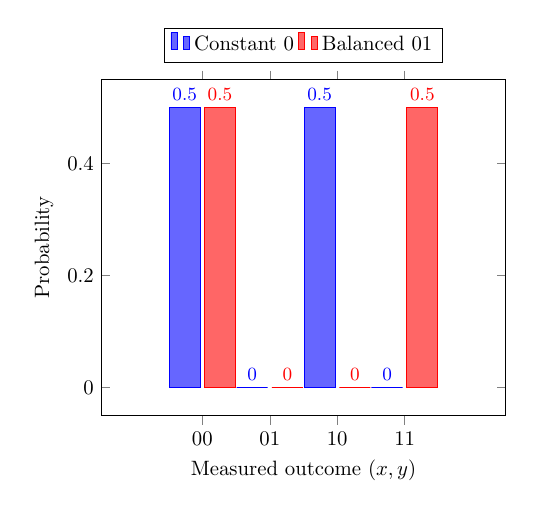
\begin{tikzpicture}[scale=.75]
\begin{axis}[
	ybar,
	bar width=15pt,
	enlarge x limits=0.5,
	ylabel={Probability},
	xlabel={Measured outcome $(x,y)$},
	symbolic x coords={00,01,10,11},
	xtick=data,
	nodes near coords,
	every node near coord/.append style={font=\small},
	legend style={at={(0.5,1.05)}, anchor=south,legend columns=-1},
	]
	% constant 0 oracle: f(0)=f(1)=0
	\addplot+[fill=blue!60] coordinates {
		(00,0.5) (01,0)   (10,0.5) (11,0)
	};
	% balanced 01 oracle: f(0)=0,f(1)=1
	\addplot+[fill=red!60]  coordinates {
		(00,0.5) (01,0)   (10,0)   (11,0.5)
	};
	\legend{Constant $0$, Balanced $01$}
\end{axis}
\end{tikzpicture}
\end{minipage}
\end{center}
\end{example}

\newpage
\begin{example}
Given $U_f:\C^4\to \C^4:\ket{x,y}\mapsto\ket{x,y\oplus f(x)}$, consider: \begin{center}
	\begin{quantikz}[column sep=.5cm]
		\lstick{$\ket{-}$} & \qw                              &\gate[2]{U_f} & \qw & \push{\scriptstyle \ket{-}\oplus f(H\ket{+})} \qw\slice{\scriptsize $U_f\ket{+,-}$} & \qw \\
		\lstick{$\ket{+}$} & \push{\scriptstyle H\ket{+}} \qw &              & \qw & \push{\scriptstyle H\ket{+}} \qw & \qw
	\end{quantikz}
\end{center} Then 
\begin{align*}
	\ket{+,-} &= H\ket{0}\otimes H\ket{1} = H\ket{0}\otimes H(X \ket{0}), \\
	\ket{+,-} &= \left(\frac{\ket{0}+\ket{1}}{\sqrt{2}}\right)\otimes\left(\frac{\ket{0}-\ket{1}}{\sqrt{2}}\right) = \frac{1}{2}\left(\ket{00}-\ket{01}+\ket{10}-\ket{11}\right),
\end{align*} and so \[
U_f\ket{+,-} = \frac{1}{2}\left(U_f\ket{00}-U_f\ket{01}+U_f\ket{10}-U_f\ket{11}\right),
\] where \begin{align*}
	U_f\ket{00} &= \ket{0,0\oplus f(0)} &=(1-f(0)){\color{cyan}\ket{00}}+f(0){\color{magenta}\ket{01}}, \\
	U_f\ket{01} &= \ket{0,1\oplus f(0)} &=f(0){\color{cyan}\ket{00}}+(1-f(0)){\color{magenta}\ket{01}}, \\
	U_f\ket{10} &= \ket{1,0\oplus f(1)} &=(1-f(1)){\color{teal}\ket{10}}+f(1){\color{orange}\ket{11}}, \\
	U_f\ket{11} &= \ket{1,1\oplus f(1)} &=f(1){\color{teal}\ket{10}}+(1-f(1)){\color{orange}\ket{11}}.
\end{align*}
Thus, we have \begin{align*}
U_f\ket{+,-} &= \frac{1}{2}\left(U_f\ket{00}-U_f\ket{01}+U_f\ket{10}-U_f\ket{11}\right)\\
&=\frac{1}{2}\left[(1-2f(0)){\color{cyan}\ket{00}}
+(f(0)-(1-f(0))){\color{magenta}\ket{01}}
+(1-2f(1)){\color{teal}\ket{10}}
+(f(1)-(1-f(1))){\color{orange}\ket{11}}
\right] \\
&=\frac{1}{2}\left[(1-2f(0)){\color{cyan}\ket{00}}
+(-1+2f(0)){\color{magenta}\ket{01}}
+(1-2f(1)){\color{teal}\ket{10}}
+(-1+2f(1)){\color{orange}\ket{11}}
\right] \\
&=\frac{1}{2}\left[(1-2f(0))({\color{cyan}\ket{00}}-{\color{magenta}\ket{01}})
+(1-2f(1))({\color{teal}\ket{10}}-{\color{orange}\ket{11}})
\right] \\
&=\frac{1}{2}\left[
(1-2f(0))\ket{0}\otimes(\ket{0}-\ket{1})+(1-2f(1))\ket{1}\otimes(\ket{0}-\ket{1})
\right]\\
&=\frac{1}{\sqrt{2}}\left[
(1-2f(0))\ket{0}+(1-2f(1))\ket{1}
\right]\otimes\frac{(\ket{0}-\ket{1})}{\sqrt{2}}\\
&=\frac{1}{\sqrt{2}}\left[
(1-2f(0))\ket{0}+(1-2f(1))\ket{1}
\right]\otimes\ket{-}.
\end{align*}
\end{example}

\newpage
\begin{example}
Given $U_f:\C^4\to \C^4:\ket{x,y}\mapsto\ket{x,y\oplus f(x)}$, consider $U_f(H\ket{0},\ket{0})$: \begin{center}
\begin{quantikz}[column sep=.5cm]
\lstick{$\ket{1}$} &\gate{H} & \push{\scriptstyle H\ket{1}=\ket{-}} \qw &\gate[2]{U_f} & \qw &\qw                    &\push{\scriptstyle \ket{-}\oplus f(\ket{+})} \qw\slice{\scriptsize $(H\otimes I)U_f(H\otimes H)\ket{01}$} & \qw \\
\lstick{$\ket{0}$} &\gate{H} & \push{\scriptstyle H\ket{0}=\ket{+}} \qw &              & \push{\scriptstyle \ket{+}} &\gate{H} &\push{\scriptstyle H\ket{+}} \qw & \qw
\end{quantikz}
\end{center} Then \begin{align*}
(H\otimes I)U_f\ket{+,-}&=\frac{H\otimes I}{\sqrt{2}}\left[
(1-2f(0))\ket{0}+(1-2f(1))\ket{1}
\right]\otimes\ket{-}\\
&=\frac{1}{\sqrt{2}}\left[
(1-2f(0))H\ket{0}+(1-2f(1))H\ket{1}
\right]\otimes I\ket{-} \\
&=\frac{1}{\sqrt{2}}\left[
(1-2f(0))\ket{+}+(1-2f(1))\ket{-}
\right]\otimes \ket{-} \\
&=\frac{1}{\sqrt{2}}\left[
(1-2f(0))\left(\frac{\ket{0}+\ket{1}}{\sqrt{2}}\right)+(1-2f(1))\left(\frac{\ket{0}-\ket{1}}{\sqrt{2}}\right)
\right]\otimes \ket{-} \\
&=\frac{1}{2}\left[
(1-2f(0))(\ket{0}+\ket{1})+(1-2f(1))(\ket{0}-\ket{1})
\right]\otimes \ket{-} \\
&=\frac{1}{2}\left[
(1-2f(0)+1-2f(1))\ket{0}+(1-2f(0)+1-2f(1))\ket{1}
\right]\otimes \ket{-} \\
&=\left[
(1-f(0)-f(1))\ket{0}+(1-f(0)-f(1))\ket{1}
\right]\otimes \ket{-},
\end{align*} and so \begin{align*}
(H\otimes I)U_f(H\otimes H)\ket{0,1} &= (H\otimes I)U_f\ket{+,-}\\
&= \left[
(1-f(0)-f(1))\ket{0}+(1-f(0)-f(1))\ket{1}
\right]\otimes \ket{-}.
\end{align*}
Let 
\[
\ket{\psi_{\rm in}}
=(H\otimes H)\ket{0,1}
=\ket{+}\otimes\ket{-},
\]
and let 
\[
\ket{\psi'}
=U_f\,\ket{\psi_{\rm in}}
=\frac1{2}\Bigl((-1)^{f(0)}\ket{0,0}
-(-1)^{f(0)}\ket{0,1}
+(-1)^{f(1)}\ket{1,0}
-(-1)^{f(1)}\ket{1,1}\Bigr).
\]
\begin{center}
\begin{quantikz}[column sep=.5cm]
	\lstick{$\ket{1}$} &\gate{H} &\gate[2]{U_f} & \qw &\qw\slice{\scriptsize $\ket{\psi_{\rm out}}$} & \qw &\qw\rstick{$\ket{-}$}\\
	\lstick{$\ket{0}$} &\gate{H} &             &\gate{H} &\qw & \meter{} &\qw
\end{quantikz}
\end{center}
Then applying \(H\) to the first qubit yields
\[
\ket{\psi_{\rm out}}
=(H\otimes I)\,\ket{\psi'}
=\begin{cases}
	(-1)^{f(0)}\,\ket{0}\otimes\ket{-}, 
	&\text{if }f(0)=f(1)\;\text{(constant)},\\[6pt]
	(-1)^{f(0)}\,\ket{1}\otimes\ket{-}, 
	&\text{if }f(0)\neq f(1)\;\text{(balanced)}.
\end{cases}
\]
In particular, up to the irrelevant global phase \((-1)^{f(0)}\), the final state is 
\(\ket{0}\otimes\ket{-}\) exactly when \(f\) is constant, and \(\ket{1}\otimes\ket{-}\) exactly when \(f\) is balanced.

\end{example}


\newpage
%\begin{proposition}[Action of the Two‐Qubit Oracle on Standard States]
%	Let 
%	\[
%	\mathcal H = \mathbb C^2\otimes\mathbb C^2,
%	\]
%	with computational basis \(\{\ket{x}\otimes\ket{y}\mid x,y\in\{0,1\}\}\).  Given a Boolean function 
%	\(f:\{0,1\}\to\{0,1\}\), the oracle unitary 
%	\[
%	U_f:\mathcal H\to\mathcal H,\qquad
%	U_f(\ket{x}\otimes\ket{y})=\ket{x}\otimes\ket{y\oplus f(x)},
%	\]
%	can be written as
%	\[
%	U_f
%	=\sum_{x\in\{0,1\}}
%	\ket{x}\!\bra{x}\;\otimes\;X^{\,f(x)},
%	\]
%	where \(X\) is the Pauli–\(X\) (NOT) gate and \(X^0=I\), \(X^1=X\).
%	
%	In particular, when the first qubit is prepared in \(\ket{0}\) and the second qubit in one of 
%	\(\{\ket0,\ket1,\ket+,\ket-\}\), the action of \(U_f\) is as follows:
%	\[
%	\begin{aligned}
%		U_f\bigl(\ket{0}\otimes\ket{0}\bigr)
%		&=\ket{0}\otimes X^{f(0)}\ket{0}
%		=\ket{0}\otimes\ket{f(0)},\\
%		U_f\bigl(\ket{0}\otimes\ket{1}\bigr)
%		&=\ket{0}\otimes X^{f(0)}\ket{1}
%		=\ket{0}\otimes\ket{1\oplus f(0)},\\
%		U_f\bigl(\ket{0}\otimes\ket{+}\bigr)
%		&=\ket{0}\otimes X^{f(0)}\ket{+}
%		=\ket{0}\otimes\ket{+},\\
%		U_f\bigl(\ket{0}\otimes\ket{-}\bigr)
%		&=\ket{0}\otimes X^{f(0)}\ket{-}
%		=\;(-1)^{f(0)}\,\ket{0}\otimes\ket{-}.
%	\end{aligned}
%	\]
%	Thus the oracle both encodes the classical bit‐flip \(y\mapsto y\oplus f(0)\) on \(\ket0,\ket1\) and imparts the phase kick‐back \((\-1)^{f(0)}\) on the Hadamard eigenstate \(\ket-\).\qedhere
%\end{proposition}

\newpage
\subsection{Algorithm}
\begin{note}
Note that \begin{enumerate}
	\item Initialize two qubits in $\ket{0}\otimes\ket{1}$.
	\item Apply Hadamard gates to both: $H^{\otimes2}\ket{0,1}=\ket{+,-}$.
	\item Query the oracle: $\ket{\psi_1}=U_f\ket{+,-}$.
	\item Apply $H\otimes I$, yielding $\ket{\psi_{out}}=(H\otimes I)\ket{\psi_1}$.
	\item Measure the first qubit in the computational basis.
\end{enumerate}
%Writing $\ket{+}=\tfrac1{\sqrt2}(\ket0+\ket1)$ and $\ket{-}=\tfrac1{\sqrt2}(\ket0-\ket1)$,
%\[
%U_f\ket{+,-}
%=\tfrac1{2}\sum_{x\in\{0,1\}}(-1)^{f(x)}\ket{x}\otimes\bigl(\ket0-\ket1\bigr).
%\]
%Since the second register remains $\ket{-}$, we focus on the first:
%\[
%(H\otimes I)U_f\ket{+,-}
%=\frac1{2}\sum_{x,y\in\{0,1\}}(-1)^{f(x)+x\cdot y}\ket{y}\otimes\ket{-}.
%\]
%The amplitude of $\ket0$ is
%\(\displaystyle\frac12\bigl[(-1)^{f(0)}+(-1)^{f(1)}\bigr]\),
%which equals $\pm1$ if $f$ is constant and $0$ if balanced.  Thus measuring the first qubit yields 0 for constant and 1 for balanced with certainty.
\end{note}

\paragraph{Implementation of Deutsch Algorithm}
\ \\
%\begin{center}
%\begin{quantikz}[column sep=.5cm]
%	\lstick{\texttt{q[0]}} &\slice{\scriptsize \texttt{t0}} &\qw\slice{\scriptsize \texttt{t1}} &\targ{} &\gate{H}\slice{\scriptsize\texttt{t2}}  &\gate[2]{U_f} & \qw \slice{\scriptsize \texttt{t4}} & \qw      &\qw\\
%	\lstick{\texttt{q[1]}} &                                &\gate{H}                           &\qw                                              &\qw  &        &\gate{H}                       & \meter{} &\qw
%\end{quantikz}
%\end{center}
\begin{lstlisting}
@:~$ !pip install qiskit qiskit-ibm-runtime pylatexenc qiskit_aer
\end{lstlisting}

\begin{lstlisting}[style=python]
from qiskit import QuantumCircuit, QuantumRegister, ClassicalRegister  # Qiskit imports
from numpy import random  # random number generator

def deutsch_oracle_circuit():  # Deutsch oracle builder
	qy = QuantumRegister(1, 'y')  # output qubit
	qx = QuantumRegister(1, 'x')  # input qubit
	qc = QuantumCircuit(qy, qx)  # init 2-qubit circuit
	
	random.seed()  # seed RNG
	f = random.randint(4)  # choose f in {0,1,2,3}
	print('random number : ', f)  # debug print
	
	if f == 0: 
		pass # f=0: do nothing 
	elif f == 1: 
		qc.x(qy) # f=1: flip y 
	elif f == 2: 
		qc.cx(qx, qy) # f=2: CNOT x->y 
	else:
		# f=3: X-CNOT-X on x 
		qc.x(qx)
		qc.cx(qx, qy)
		qc.x(qx)  
	
	qc.name = 'Deutsch'  # label circuit
	return qc  # return oracle

circuit = deutsch_oracle_circuit()  # build oracle
circuit.draw(output='mpl')  # draw with matplotlib
\end{lstlisting}
\begin{lstlisting}
random number :  3
\end{lstlisting}
\begin{figure}[h!]\centering
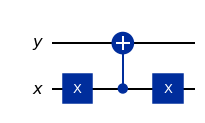
\includegraphics[scale=.5]{images/lab03_1}
\end{figure}
\begin{lstlisting}[style=python]
qx = QuantumRegister(1, 'x')    # input qubit
qy = QuantumRegister(1, 'y')    # output qubit
c  = ClassicalRegister(1, 'c')  # classical bit

circuit = QuantumCircuit(qy, qx, c)
circuit.h(qx)                   # superpose input
circuit.x(qy)                   # prepare output in |1>
circuit.h(qy)                   # superpose output
circuit.barrier()               # separate stages
oracle = deutsch_oracle_circuit()
circuit.compose(oracle, [qy[0], qx[0]], inplace=True)  # apply oracle
circuit.barrier()               # separate stages
circuit.h(qx)                   # interference on input

circuit.measure(qx, c)          # measure input
circuit.draw(output='mpl')      # visualize circuit
\end{lstlisting}
\begin{lstlisting}
random number :  3
\end{lstlisting}
\begin{figure}[h!]\centering
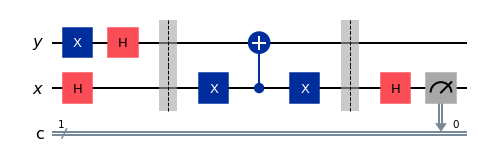
\includegraphics[scale=.5]{images/lab03_2}
\end{figure}
\begin{lstlisting}[style=python]
# simulate circuit with AerSimulator and print counts
from qiskit.transpiler.preset_passmanagers import generate_preset_pass_manager
from qiskit_ibm_runtime import SamplerV2 as Sampler
from qiskit_aer import AerSimulator

aer_sim = AerSimulator()  # create simulator
pm = generate_preset_pass_manager(backend=aer_sim, optimization_level=1) 

isa_circuit = pm.run(circuit)  # transpile circuit
sampler = Sampler(mode=aer_sim)  # create sampler
job = sampler.run([isa_circuit], shots=1)  # run circuit once
result = job.result()  # get results
count = result[0].data.c.get_counts()  # extract counts
print(count)  # print counts
\end{lstlisting}
\begin{lstlisting}
{'1': 1}
\end{lstlisting}
\begin{lstlisting}[style=python]
if ('0' in count) :
	answer = 'constant'
else :
	answer = 'balanced'

print (f'f(x) is a {answer} function.')
\end{lstlisting}
\begin{lstlisting}
f(x) is a balanced function.
\end{lstlisting}

\newpage
\section{Phase Kickback}\label{sec:phase-kickback}

In many quantum algorithms, such as Deutsch, Deutsch--Jozsa, and Bernstein--Vazirani, the \emph{phase kickback} effect allows one to encode information about a Boolean function $f$ into relative phases of a register.  We present here a rigorous derivation and formal statement of phase kickback.

\subsection{Oracle Unitary and Hadamard Eigenstate}
Let $f:\{0,1\}^n\to\{0,1\}$ be a Boolean function, and define the \emph{oracle unitary}
\[
U_f:\mathbb C^{2^n}\otimes\mathbb C^2 \to \mathbb C^{2^n}\otimes\mathbb C^2,
\quad
U_f\bigl(\ket{x}\otimes\ket{y}\bigr)=\ket{x}\otimes\ket{y\oplus f(x)},
\]
where $x\in\{0,1\}^n$, $y\in\{0,1\}$.  As shown in Section~\ref{sec:oracle-def}, $U_f$ is unitary and acts on the second qubit by a conditional bit‐flip.

Define the Hadamard eigenstates on the second qubit:
\[
\ket{+}=H\ket{0}=\tfrac1{\sqrt2}(\ket{0}+\ket{1}),
\qquad
\ket{-}=H\ket{1}=\tfrac1{\sqrt2}(\ket{0}-\ket{1}).
\]

\begin{lemma}[Phase Kickback]
	For any $x\in\{0,1\}^n$, the oracle unitary satisfies
	\[
	U_f\bigl(\ket{x}\otimes\ket{-}\bigr)
	=\ket{x}\otimes X^{f(x)}\ket{-}
	= (-1)^{f(x)}\,\ket{x}\otimes\ket{-}.
	\]
\end{lemma}

\begin{proof}
	Since $X\ket{-}=-\ket{-}$ and $X^0=I$, we have
	\[
	X^{f(x)}\ket{-}
	=\begin{cases}
		\ket{-}, & f(x)=0, \\
		-\ket{-}, & f(x)=1,
	\end{cases}
	= (-1)^{f(x)}\ket{-}.
	\]
	Hence
	\[
	U_f(\ket{x}\otimes\ket{-})
	= \ket{x}\otimes X^{f(x)}\ket{-}
	= (-1)^{f(x)}\ket{x}\otimes\ket{-}.
	\]
\end{proof}

\subsection{Multi‐Qubit Extension}
By linearity, an arbitrary first‐register state $\ket{\psi}=\sum_x a_x\ket{x}$ yields
\[
U_f\bigl(\ket{\psi}\otimes\ket{-}\bigr)
=\sum_{x}a_x(-1)^{f(x)}\ket{x}\otimes\ket{-}
= \bigl(V_f\ket{\psi}\bigr)\otimes\ket{-},
\]
where the \emph{phase oracle} is
\[
V_f=\sum_{x}(-1)^{f(x)}\ket{x}\bra{x}.
\]

\subsection{Applications and Remarks}
\begin{itemize}
	\item In the \emph{Deutsch} algorithm ($n=1$), one starts with $(H\otimes I)U_f(H\otimes H)\ket{0,1}$, and phase kickback yields $(H\otimes I)U_f(\ket{+}\otimes\ket{-})=\pm\ket{0}\otimes\ket{-}$ or $\pm\ket{1}\otimes\ket{-}$, distinguishing constant versus balanced cases with one final Hadamard and measurement.
	\item In \emph{Deutsch--Jozsa} and \emph{Bernstein--Vazirani}, phase kickback on an $n$‑qubit superposition imprints the global phase pattern $(-1)^{f(x)}$, subsequently decoded by an $n$‑fold Hadamard transform.
	\item The phase oracle $V_f$ acts without extra ancilla, showing that any $y$‑qubit initialized to $\ket{-}$ serves as a pure phase marker.
\end{itemize}

This completes the formal lecture notes on phase kickback, a key primitive in quantum algorithmic speed‑ups.
\newpage
\subsection{Exercises}
Consider the two‐qubit unitary evolution \[
\ket{\psi_{\rm in}}
=(H\otimes H)\ket{1,1},
\quad
\ket{\psi'}
=U_f\,\ket{\psi_{\rm in}},
\quad
\ket{\psi_{\rm out}}
=(H\otimes I)\,\ket{\psi'}.
\]
\begin{center}
\begin{quantikz}[column sep=.5cm]
	\lstick{$\ket{1}$} &\gate{H} &\gate[2]{U_f} & \qw &\qw\slice{\scriptsize $\ket{\psi_{\rm out}}$} & \qw &\qw \\
	\lstick{$\ket{1}$} &\gate{H} &             &\gate{H} &\qw & \meter{} &\qw
\end{quantikz}
\end{center}
\begin{enumerate}[(a)]
	\item Show that
	\[
	\ket{\psi_{\rm out}}
	=\frac{1}{2\sqrt2}
	\Bigl[
	(-1)^{f(0)}\ket{00}
	-(-1)^{f(0)}\ket{01}
	+(-1)^{f(1)}\ket{10}
	-(-1)^{f(1)}\ket{11}
	\Bigr],
	\]
	and hence write \(\ket{\psi_{\rm out}}\) as a linear combination of the basis
	\(\{\ket{00},\ket{01},\ket{10},\ket{11}\}\).
	\item Suppose \(f(0)=f(1)=1\).  If the first qubit (\(q_1\)) is measured in the computational basis, compute
	\(\Pr[q_1=1]\) and \(\Pr[q_1=0]\).
\end{enumerate}
\begin{proof}[\normalfont\bfseries\textcolor{magenta}{Sol}]
\textbf{(a)}\; First,
\[
\ket{\psi_{\rm in}}
= (H\otimes H)\ket{1,1}
= \ket{-}\otimes\ket{-}
= \frac1{2}\sum_{x=0}^1\ket{x}\otimes(\ket{0}-\ket{1}).
\]
By phase kickback,
\[
\ket{\psi'}
= U_f(\ket{-}\otimes\ket{-})
= \frac1{2}\sum_{x=0}^1(-1)^{f(x)}\,\ket{x}\otimes(\ket{0}-\ket{1}).
\]
Applying \(H\) on the first qubit gives
\[
\ket{\psi_{\rm out}}
=(H\otimes I)\ket{\psi'}
=\frac1{2}\sum_{x=0}^1(-1)^{f(x)}\bigl(H\ket{x}\bigr)\otimes(\ket{0}-\ket{1})
=\frac{1}{2\sqrt2}\sum_{a,x=0}^1(-1)^{ax+f(x)}\ket{a}\otimes(\ket{0}-\ket{1}),
\]
which is equivalently
\[
\boxed{
	\ket{\psi_{\rm out}}
	=\frac{1}{2\sqrt2}
	\bigl[
	(-1)^{f(0)}\ket{00}
	-(-1)^{f(0)}\ket{01}
	+(-1)^{f(1)}\ket{10}
	-(-1)^{f(1)}\ket{11}
	\bigr].
}
\]

\medskip\noindent\textbf{(b)}\; If \(f(0)=f(1)=1\), then \((-1)^{f(x)}=-1\) for \(x=0,1\).  Substituting,
\[
\ket{\psi_{\rm out}}
=\frac{-1}{2\sqrt2}
\bigl[\ket{00}-\ket{01}+\ket{10}-\ket{11}\bigr]
=\frac{-1}{\sqrt2}\bigl(\ket{00}-\ket{01}\bigr).
\]
Thus the only nonzero amplitudes are on \(\ket{00}\) and \(\ket{01}\), each of magnitude \(1/\sqrt2\).  Consequently,
\[
\Pr[q_1=0]
=\left(-\frac{1}{\sqrt{2}}\right)^2
+\left(-\frac{1}{\sqrt{2}}\right)^2
=\frac12+\frac12=1,
\quad
\Pr[q_1=1]=0.
\]
This completes the solution.
\end{proof}


\newpage
\section{Deutsch--Jozsa Algorithm}
\label{sec:DeutschJozsa}
\subsection{Problem Statement}
Generalize to $f:\{0,1\}^n\to\{0,1\}$ promised either
\begin{itemize}
	\item \emph{constant}: $f(x)$ same for all $x$, or
	\item \emph{balanced}: $f(x)=0$ for exactly $2^{n-1}$ inputs,
\end{itemize}
Classically requires $2^{n-1}+1$ evaluations in worst case; quantum requires one.

\subsection{Algorithm Steps}
\begin{enumerate}
	\item Prepare $n+1$ qubits in $\ket{0}^{\otimes n}\otimes\ket{1}$.
	\item Apply $H^{\otimes(n+1)}$, yielding
	$\ket{\psi_1}=\tfrac1{2^{n/2}}\sum_{x}\ket{x}\otimes\ket{-}$.
	\item Oracle: $\ket{\psi_2}=U_f\ket{\psi_1}=\tfrac1{2^{n/2}}\sum_x(-1)^{f(x)}\ket{x}\otimes\ket{-}$.
	\item Apply $H^{\otimes n}\otimes I$, obtaining
	\[
	\ket{\psi_{out}}=\frac1{2^n}\sum_{y,x}(-1)^{f(x)+x\cdot y}\ket{y}\otimes\ket{-}.
	\]
	\item Measure the first $n$ qubits.
\end{enumerate}

\subsection{Analysis}
The amplitude on $\ket{0^n}$ is \(\displaystyle\frac{1}{2^n}\sum_x(-1)^{f(x)}\),
which equals $\pm1$ if $f$ is constant and $0$ if balanced.  A single measurement thus solves the problem with certainty.

%\subsection{Circuit Diagram}
%\[
%\begin{quantikz}
%	\lstick{\ket{0}^{\otimes n}} & \gate{H}^{\otimes n} & \ctrl{n} & \gate{H}^{\otimes n} & \meter{}\\
%	\lstick{\ket1}               & \gate{H}             & \targ{}  & \qw                   & \qw
%\end{quantikz}
%\]

\newpage
\begin{lstlisting}[style=python]
from qiskit import QuantumCircuit, QuantumRegister, ClassicalRegister  # imports
import numpy as np  # numpy

def dj_oracle_random(n):  # random n-qubit DJ oracle
	qy = QuantumRegister(1, 'y')       # y qubit
	qx = QuantumRegister(n, 'x')       # x qubits
	qc = QuantumCircuit(qy, qx)        # init circuit
	
	np.random.seed()                   # seed RNG
	condition = np.random.choice(['constant', 'balanced'])  # oracle type
	print(condition)                   # debug
	
	if condition == 'constant':        # constant case
		x = np.random.randint(2)       # output bit
		print(x)                       # debug
		# if x==1 f(x)=1, if x==0 f(x)=0
		if x == 1:
			qc.x(qy)                   # flip y
	else:                              # balanced case
		k = np.random.randint(1, n+1)       # number of flips
		a = np.random.permutation(n)        # permute indices
		a = a[:k]                           # take first k indices
		print(a)                            # debug
		for idx in a:
			qc.cx(qx[idx], qy[0])          # CNOT x->y
	
	qc.name = 'D-Jozsa'                # set name
	return qc                          # return oracle

circuit = dj_oracle_random(7)        # build oracle
circuit.draw(output='mpl')           # draw circuit
\end{lstlisting}
\begin{lstlisting}
balanced
[5 2 6 4 1 0 3]
\end{lstlisting}

\begin{figure}[h!]\centering
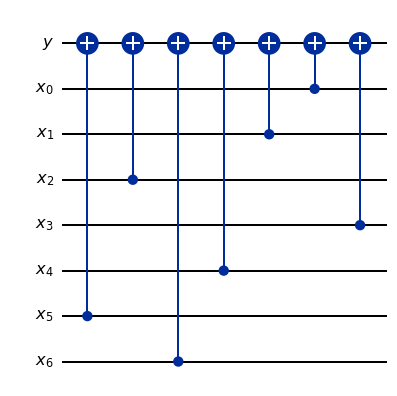
\includegraphics[scale=.5]{images/lab04_1}
\end{figure}

\begin{lstlisting}[style=python]
n = 7
qx = QuantumRegister(n, 'x')                 # input qubits
qy = QuantumRegister(1, 'y')                 # ancilla qubit
c  = ClassicalRegister(n, 'c')               # classical bits
circuit = QuantumCircuit(qy, qx, c)          # init circuit
for qubit in qx:
circuit.h(qubit)                           # H on all x qubits
circuit.x(qy)                                # X on y
circuit.h(qy)                                # H on y
circuit.barrier()                            # barrier
oracle_circuit = dj_oracle_random(n)         # build oracle
circuit.compose(oracle_circuit, qubits=[*qy, *qx], inplace=True)  # apply oracle
circuit.barrier()                            # barrier
for qubit in qx:
	circuit.h(qubit)                           # H on all x qubits
for i in range(n):
	circuit.measure(qx[i], c[i])               # measure x into c
circuit.draw(output='mpl')                   # draw circuit
\end{lstlisting}
\begin{lstlisting}
balanced [0 5 1 4]
\end{lstlisting}

\begin{figure}[h!]\centering
	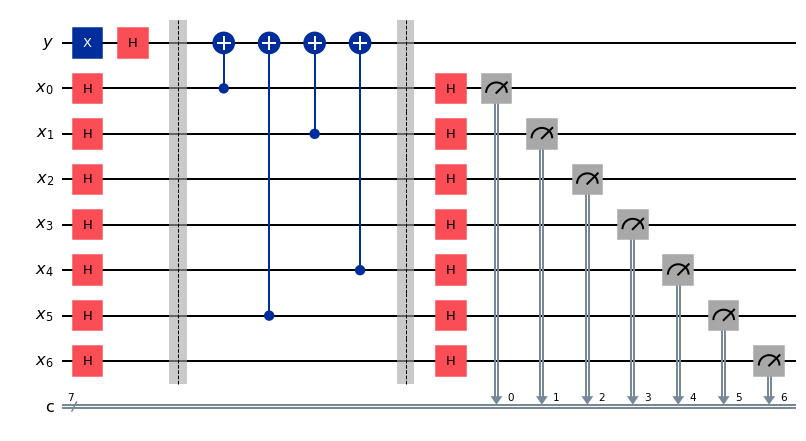
\includegraphics[scale=.5]{images/lab04_2}
\end{figure}

\begin{lstlisting}[style=python]
from qiskit.transpiler.preset_passmanagers import generate_preset_pass_manager
from qiskit_ibm_runtime import SamplerV2 as Sampler
from qiskit_aer import AerSimulator
aer_sim = AerSimulator()
pm = generate_preset_pass_manager(backend=aer_sim, optimization_level=1)
isa_circuit = pm.run(circuit)
sampler = Sampler(mode=aer_sim)
job = sampler.run([isa_circuit], shots=1)
result = job.result()
count = result[0].data.c.get_counts()
print (count)
\end{lstlisting}
\begin{lstlisting}
{'0110011': 1}
\end{lstlisting}

\begin{lstlisting}[style=python]
n_zeros = n*'0'
if (n_zeros in count) : answer = 'constant'
else : answer = 'balanced'
print(f'f(x) is a {answer} function.')
\end{lstlisting}
\begin{lstlisting}
f(x) is a balanced function.
\end{lstlisting}


\newpage
\section{Bernstein--Vazirani Algorithm}
\label{sec:BernsteinVazirani}
\subsection{Problem Statement}
Given oracle access to $f_s(x)=s\cdot x\pmod2$ for unknown $s\in\{0,1\}^n$, determine $s$.  Classically requires $n$ queries; quantum uses one.

\subsection{Algorithm}
\begin{enumerate}
	\item Initialize $\ket{0}^{\otimes n}\otimes\ket1$.
	\item Apply $H^{\otimes(n+1)}$: get $\tfrac1{\sqrt{2^n}}\sum_x\ket{x}\otimes\ket{-}$.
	\item Oracle: $\ket{\psi_2}=\tfrac1{\sqrt{2^n}}\sum_x(-1)^{s\cdot x}\ket{x}\otimes\ket{-}$.
	\item Apply $H^{\otimes n}\otimes I$: by Fourier analysis,
	\[
	(H^{\otimes n}\sum_x(-1)^{s\cdot x}\ket{x})\otimes\ket{-}
	=\ket{s}\otimes\ket{-}.
	\]
	\item Measure first $n$ qubits to read out $s$.
\end{enumerate}

\subsection{Proof of Correctness}
Using $H^{\otimes n}\ket{x}=\tfrac1{2^{n/2}}\sum_y(-1)^{x\cdot y}\ket{y}$, we compute
\[
H^{\otimes n}\Bigl(\sum_x(-1)^{s\cdot x}\ket{x}\Bigr)
=\sum_y\frac1{2^{n/2}}\sum_x(-1)^{s\cdot x + x\cdot y}\ket{y}
=\ket{s},
\]
%as the inner sum vanishes unless $y=s$.  Thus measurement yields $s$ with unit probability citeturn2file4.

\section*{Exercises}
\begin{enumerate}
	\item Prove phase‐kickback more generally: for any $f:\{0,1\}^n\to\{0,1\}$,
	show $U_f(\ket{x}\otimes\ket{-})=(-1)^{f(x)}\ket{x}\otimes\ket{-}$.
	\item Extend Deutsch--Jozsa to detect whether $f$ has Hamming weight $k$.
	\item Analyze robustness of Bernstein--Vazirani against depolarizing noise.
\end{enumerate}

\newpage
\begin{lstlisting}[style=python]
from qiskit import QuantumCircuit, QuantumRegister, ClassicalRegister  # Qiskit imports
import numpy as np  # numpy import

# BV oracle builder
	def bv_oracle_circuit(n, reveal=False):
	qy = QuantumRegister(1, 'y')          # y qubit
	qx = QuantumRegister(n, 'x')          # x qubits
	qc = QuantumCircuit(qy, qx)           # init circuit
	np.random.seed()                      # seed RNG
	s = list(np.random.randint(0, 2, size=n))  # random secret
	if reveal: print("random binary string =", s)  # debug print
	for i in range(n):
		if s[i]:                          # secret bit check
			qc.cx(qx[i], qy[0])          # CNOT x->y
	qc.name = "BV Oracle"                # label circuit
	hs = ''
	for c in reversed(s):
		hs += str(c)                     # build string
	return qc, hs                         # return circuit, secret

circuit, hs = bv_oracle_circuit(5, True)  # build oracle
circuit.draw(output='mpl')               # draw circuit

\end{lstlisting}
\begin{lstlisting}
random binary string =  [1, 1, 1, 0, 1].
\end{lstlisting}

\begin{figure}[h!]\centering
	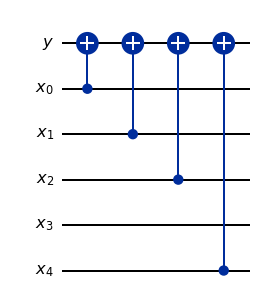
\includegraphics[scale=.5]{images/lab05_1}
\end{figure}

\begin{lstlisting}[style=python]
# build Bernstein-Vazirani circuit
n = 8
qx = QuantumRegister(n, 'x')          # input qubits
qy = QuantumRegister(1, 'y')          # ancilla qubit
c  = ClassicalRegister(n, 'c')        # classical bits
circuit = QuantumCircuit(qy, qx, c)   # init circuit
circuit.h(qx)                         # H on x
circuit.x(qy)                         # X on y
circuit.h(qy)                         # H on y
circuit.barrier()                     # barrier
oracle, hs = bv_oracle_circuit(n, reveal=True)           # build oracle
print(f'hidden string = {hs}')                          # show secret
circuit.compose(oracle, qubits=[qy[0]] + list(qx), inplace=True)  # apply oracle
circuit.barrier()                     # barrier
circuit.h(qx)                         # H on x
circuit.measure(qx, c)                # measure x to c
circuit.draw(output='mpl')            # draw circuit
\end{lstlisting}
\begin{lstlisting}
random binary string =  [1, 1, 0, 1, 1, 0, 1, 1]
hidden string = 11011011
\end{lstlisting}

\begin{figure}[h!]\centering
	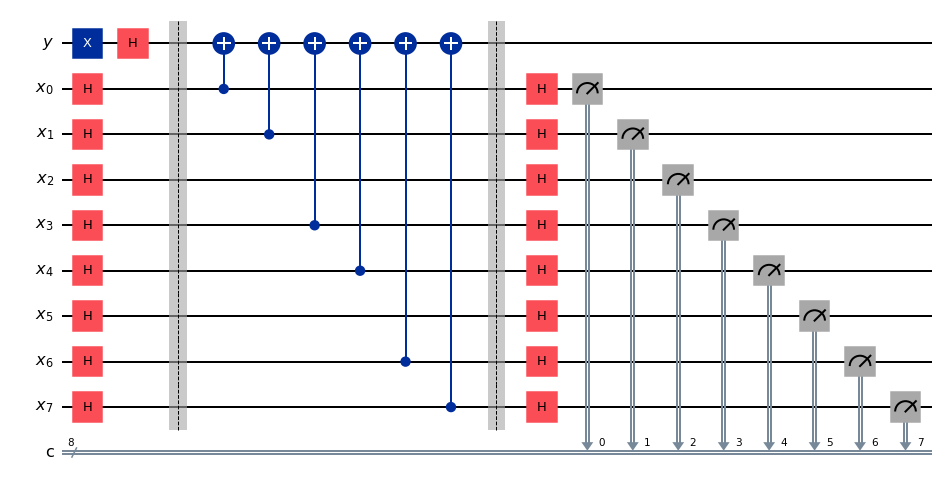
\includegraphics[scale=.5]{images/lab05_2}
\end{figure}

\begin{lstlisting}[style=python]
from qiskit.transpiler.preset_passmanagers import generate_preset_pass_manager
from qiskit_ibm_runtime import SamplerV2 as Sampler
from qiskit_aer import AerSimulator

aer_sim = AerSimulator()
pm = generate_preset_pass_manager(backend=aer_sim, optimization_level=1)

isa_circuit = pm.run(circuit)
sampler = Sampler(mode=aer_sim)
job = sampler.run([isa_circuit], shots=1)
result = job.result()
count = result[0].data.c.get_counts()
print (count)
\end{lstlisting}
\begin{lstlisting}
{'11011011': 1}
\end{lstlisting}

\begin{lstlisting}[style=python]
measured = list(count.keys())[0]

print (f'The measured value {measured} ', end='')
if hs == measured :
	print(f'is equal to the hidden string {hs}')
else :
	print(f'is not equal to the hidden string {hs}')
\end{lstlisting}
\begin{lstlisting}
The measured value 11011011 is equal to the hidden string 11011011
\end{lstlisting}



